\documentclass[12pt]{article}
%\usepackage{apacite}
\usepackage{wrapfig}
\setlength{\parindent}{0pt}
\usepackage{caption} %test
\captionsetup[figure]{font=small} %test
\usepackage{tgtermes}
\usepackage{setspace}
\usepackage{gensymb}
\usepackage{amsmath}
\usepackage{hyperref}
\doublespacing
\usepackage{graphicx}
\usepackage{float}
\usepackage[utf8]{inputenc}
\usepackage[backend=biber,style=apa,autocite=inline]{biblatex}
\usepackage{fancyhdr}
\pagestyle{fancy}
\lhead{Affective weighting function}
\rhead{Victor M. Poulsen, Studie Nr.: 201707639}

\DeclareLanguageMapping{english}{english-apa}
\addbibresource{References.bib}
\setcounter{page}{1}

\title{Affective modulation of the weighting function}
\author{Victor Møller Poulsen, Studie Nr.: 201707639}

\begin{document}
\maketitle
\leavevmode

\textbf{Code}: Simulation, figures and
full analysis pipeline available at: \\
\href{https://github.com/victor-m-p/BayesianDecisionWeights}
{https://github.com/victor-m-p/BayesianDecisionWeights}

\tableofcontents

\section{Description}

For decisions under uncertainty
(e.g. bets), decision theories
(e.g. Prospect Theory) can explain the
value assigned to bets by combining two functions
\autocite{rottenstreich2001money}.
A value function $v$ transforms objective value to
subjective utility, and a probability
weighting function $w$
distorts probabilities \autocite{rottenstreich2001money,
gonzalez1999shape}.
In prospect theory (PT)
and expected-utility theory (EUT) the two parameters
are combined in
the simplest way possible
\autocite{rottenstreich2001money}

\[
	\sum w(p_i)v(i),
\]

where $p$ stands for probability and $i$ stands for the
$i^{th}$ gamble. \\

That decision making under uncertainty can
be formalized as a combination of a value
function $v$ and a weight function  $w$
can be construed
as either an "as-if" or a "process" model
\autocite{newell2015straight}. Where the
"as-if" model simply claims that people act
"as-if" these functions are computed, and the
process model claims that people actually compute
these functions (or something similar). This
is not a primary concern here. \\

In EUT the weight function $w$
is the identity $w(p) = p$, assuming that people do
not distort probabilities \autocite{rottenstreich2001money}.
Further, in EUT the value functin $v$ is
proposed to reflect how people feel about
the utility of end states. This assumes that people should
take into account their current state (e.g. of wealth)
when evaluating outcomes
\autocite{newell2015straight}.

\vspace{3mm}

With regards to both the value function $v$ and
the weight function $w$,
PT \autocite{
	PT,
tversky1992advances} advances theorizing,
and better explains empirical results
\autocite{abdellaoui2010separating,
wu1996curvature} as compared to EUT.
PT is arguably the main model of human decision making
\autocite{newell2015straight}.
PT advances theorizing
with regards to the value function $v$
by positing that losses and
gains are evaluated as changes in wealth rather
than with regards to end states. This means that
in a monetary domain, rich and poor people
should show relatively similar
behaviour. This is because both will
evaluate outcomes based
on a neutral reference point (i.e. not
changing from the status quo)
\autocite{newell2015straight,
abdellaoui2010separating}.
This leads us to the familiar (non-linear) S-shaped
value function $v$ proposed in PT \autocite{PT}.
The value function $v$ is concave for the gains
domain and convex for the loss domain.
This reflects the
fact that small changes in outcome are relatively
overweighted close to the status quo as
compared to far away from the status quo.
A monetary increase from
$0 - 100\$$ has greater subjective utility
than an increase
from $1000 - 1100\$$, although the latter
increase in wealth is identical in absolute terms.
The same is the case for the
domain of losses, where small increments are
relatively overweighted close to the
status quo. Another key stylistic of the
value function is that it is steeper for the
loss domain than for the gains domain
\autocite{newell2015straight}.
A majority of people will not take an gamble
with a $0\$$ expected value (e.g.  $50\%$ chance
to lose  $100\$$ and a  $50\%$ chance to win
$100\$$). This is the famous loss aversion. \\

PT advances theorizing with regards to
the weight function $w$
by allowing a (non)-linear probability
distortion \autocite{PT,
gonzalez1999shape}. $w$ is stylized as
being reverse S-shaped, meaning that it is
concave for low probabilities and convex for
high probabilities \autocite{gonzalez1999shape,
wu1996curvature}.
This means that
people underweight changes in probability in
the middle of the spectrum (e.g. $[0.2-0.8]$)
while overweighting changes in probability close
to the end-points (e.g. $[0.0 - 0.2], [0.8 - 1.0]$).
These general characteristics of the weighting
function are empirically well documented
\autocite{tversky1992advances,
wu1996curvature,
abdellaoui2010separating}.
Prospect theory (PT) also allows for potentially
different weighting functions for gains $w^{+}$
and losses  $w^{-}$ \autocite{abdellaoui2010separating}.
Generally, the probability weighting function $w$
has received less attention than the value function
$v$ \autocite{gonzalez1999shape}.

\subsection{Prior work}

There is evidence to support
the notion that the affect-richness of outcomes modulates
the parameters of both the value function $v$
\autocite{hsee2004music} and the weight functon $w$
\autocite{
rottenstreich2001money}. \\

The reverse S-shape (curvature) of the weighting function
$w$ appears to be more pronounced
for high-affect than low-affect outcomes under
uncertainty \autocite{rottenstreich2001money}.
\textcite{rottenstreich2001money}
investigated how much participants were
willing to pay for two coupons
(worth the same) at different
levels of probability. The first item was
a coupon redeemable for a trip to
Europe (high-affect) while the second
item was a coupon redeemable for
covering tuition fees (low-affect).
\textcite{rottenstreich2001money}
were able to show a preference reversal in
which the high-affect outcome was preferred for
low probability (1\%) whereas the low-affect
outcome was preferred for high probability (99\%).
If this result is solid, it suggests
that people distort probabilities
more for high-affect as compared to low-affect
outcomes. It also violates the probability-outcome
independence that both EUT and PT hold,
and suggests that this independence might
not hold for across outcomes which differ
in affect \autocite{rottenstreich2001money}. \\

For the gains domain, the value function $v$
has been shown to be more
concave for high-affect as opposed to low-affect
outcomes \autocite{hsee2004music}.
\textcite{hsee2004music} showed this by
priming participants to
evaluate outcomes either based on calculation or
based on feeling. Their results clearly suggest
a modulatory effect of affect-richness.
Together, the results suggest a consistent picture
of modulation of both the value function $v$ and
the weight function  $w$. This line of evidence
has been pursued elsewhere \autocite{
	mukherjee2010dual,
mukherjee2011thinking} with the idea of modeling
decision making as an interaction between an
affective system and a deliberative system.
Theoretically, the results of
\textcite{rottenstreich2001money,
hsee2004music} are consistent with the
"risk-as-feelings" hypothesis \autocite{loewenstein2001risk}
which suggests that emotional reactions
to decisions under uncertainty often diverge
from cognitive assessment. It seems plausible
that small and large probabilities of obtaining an
affect-rich outcome would elicit
comparably strong mental images and thus
comparably strong emotional reactions.

\subsection{Focus and parameterization}

In this article we focus exclusively on the
weighting function $w$ while ignoring both
the value function $v$ and the combination
of the two functions. We also restrict ourselves
to the gains domain. A weighting function
is formally a mapping from the interval
$[0, 1]$ into  $[0, 1]$ \autocite{abdellaoui2010separating}.
The probability weight function can be
empirically studied independently of
the value function \autocite{wu1996curvature}.
In \textcite{rottenstreich2001money} they
suggest that future work (building on their
stylized results) should estimate the affective
modulation on the parameter(s) of the
weighting function $w$. This is something
that they do not do in their article.
They specifically
propose that the affective modulation can
be estimated as an affect parameter $a$
in the general parameterization of the weighting
function $w$:

\[
	w(p) = \frac{p^{1-a}}
	{p^{1-a}+(1-p)^{1-a}}
.\]

where $a \in [0, 1]$ and larger $a$ values indicate
greater affect
and more curvature \autocite{rottenstreich2001money}.
The issue with this one-parameter
formulation is that it
does not account for the fact that people
generally show low \emph{elevation}.
What I mean by that is that the empirically
observed weighting function $w$ typically
crosses the diagonal line given by $w(p) = p$
at around $0.3-0.4$ rather than at $0.5$
\autocite{gonzalez1999shape,
abdellaoui2010separating,
wu1996curvature}. This can be
interpreted as people generally being
pessimistic (i.e. $50\%$ probability is
evaluated as being worth less than  $50\%$
of the outcome).
The one-parameter
formulation fixes the
cross-over point at $0.5$,
(i.e. $w(0.5) = 0.5$),
which can be seen from figure $1$.

\begin{figure}[H]
	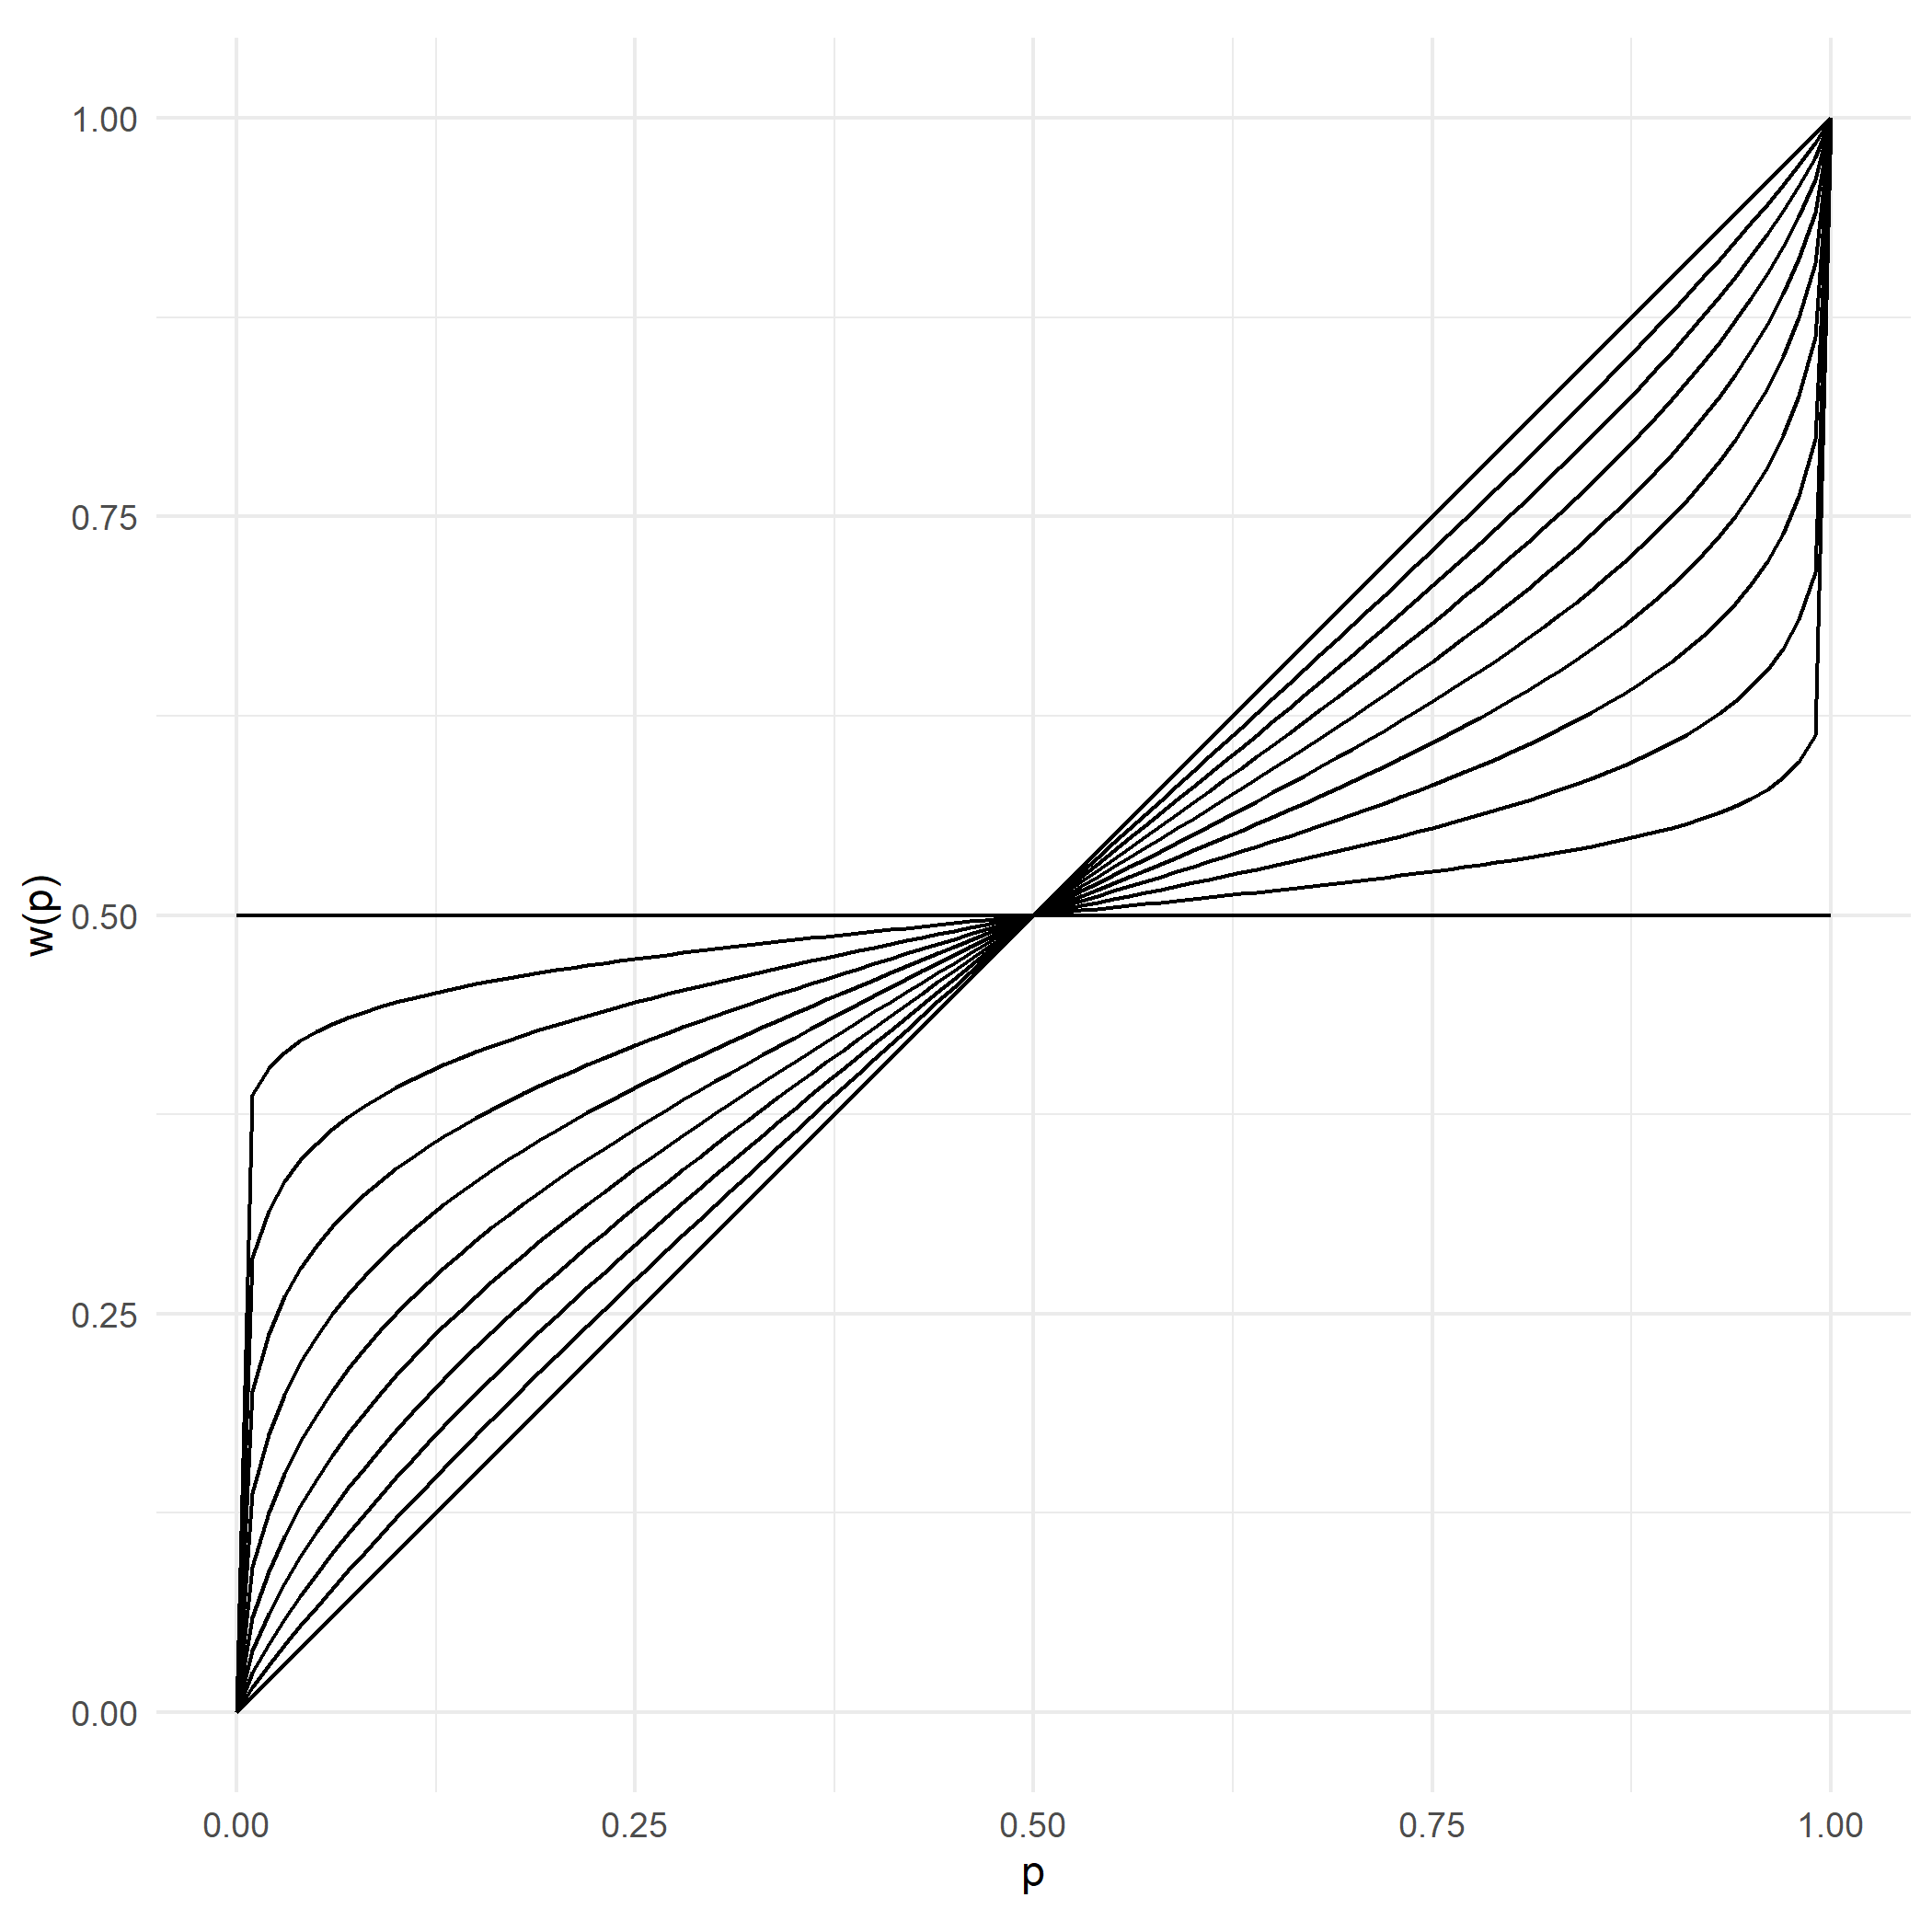
\includegraphics[width = \linewidth]{../Figures/oneParam.png}
	\caption{Data simulated from the model
		$w(p) = \frac{p^{1-a}}
		{p^{1-a}+(1-p)^{1-a}}$ with
		$a \in [0, 1]$ (see
		\href{https://github.com/victor-m-p/BayesianDecisionWeights/blob/main/Code/0_visualize_parameters.Rmd}
		{this file} on the
		\href{https://github.com/victor-m-p/BayesianDecisionWeights}{github}).
		Diagonal line has
		$a = 0$, and the horizontal line
		has $a = 1$. Intermediate curves
		are generated for $0.2$ increments
		of $a$. All values beside
		$a = 0$ show a probability distortion
		as compared to the objective probability.
		Note that all curves meet at
		$w(p) = 0.5, p = 0.5$. This is
	not empirically supported.}
\end{figure}

Instead of using the parameterization
proposed in \textcite{rottenstreich2001money}
this paper will use one of the
proposed two-parameter functions
suggested in \textcite{gonzalez1999shape}.
Specifically,
\[
	\log\frac{w(p)}{1-w(p)} =
	\gamma \log\frac{p}{1-p} + \tau
.\]

where solving for $w(p)$ and setting $\delta = \exp(\tau)$
gives us

\[
	w(p) = \frac{\delta \cdot p^{\gamma}}
	{\delta \cdot p^{\gamma} +
	(1-p)^{\gamma}}
.\]

As can be seen $w$ is parameterized with
$\delta$ and $\gamma$. Other two-parameter
forms which attempt to capture elevation and
curvature have been proposed, including the
constant relative sensitivity (CRS) weighting
functions \autocite{abdellaoui2010separating}.

\vspace{3mm}

In the formulation above, the
$\delta$ parameter will vary based on
\emph{elevation} (intercept)
\autocite{gonzalez1999shape},
which here simply refers to the overall
perceived attractiveness of outcomes
under uncertainty.

\vspace{3mm}

The $\gamma$ parameter will vary based on
\emph{curvature} (slope)
\autocite{gonzalez1999shape} and is what we
are primarily interested in for our purposes.
It follows as a direct prediction from
\textcite{rottenstreich2001money} that the
curvature ($\gamma$) should be modulated by changes in
the affective level of outcomes.
The two parameters are logically independent,
and as such they should be modeled
independently and not be collapsed into one
parameter \autocite{abdellaoui2010separating,
gonzalez1999shape}. \\

$w(p) = p$ for  $\gamma = 1$ and $\delta = 1$
with this parameterization. Empirically,
$\delta < 1$ and $\gamma < 1$
\autocite{gonzalez1999shape}. $\delta < 1$
reflects low elevation (as compared to diagonal)
and  $\gamma < 1$ reflects high curvature
(reverse S-shape). Note that the interpretation
of $\gamma$ is opposite the interpretation of
$a$ as proposed in the parameterization of
\textcite{rottenstreich2001money}. As such,
if follows from \textcite{rottenstreich2001money}
that high-affect outcomes should result in low
$\gamma$.
See figure 2 for an
illustration of how the $\delta$
and $\gamma$ parameters independently modulate
different aspects of the weighting function $w$.

\begin{figure}[H]
	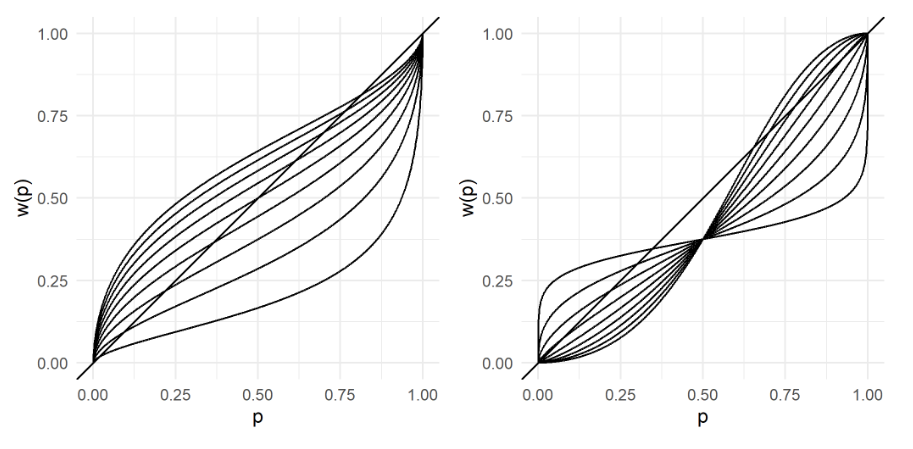
\includegraphics[width = \linewidth]{../Figures/Fig2.png}
	\caption{Data simulated from the model
		$w(p) = \frac{\delta \cdot p^{\gamma}}
	{\delta \cdot p^{\gamma} +
	(1-p)^{\gamma}}$ (see
		\href{https://github.com/victor-m-p/BayesianDecisionWeights/blob/main/Code/0_visualize_parameters.Rmd}
		{this file} on the
		\href{https://github.com/victor-m-p/BayesianDecisionWeights}{github}). The figure
	is similar to figure 4
	of \textcite{gonzalez1999shape}.
	On the left: $\gamma$ fixed at $0.6$
	and $\delta$ varied between $0.2$ and $1.8$.
	On the right: $\delta$ fixed at $0.6$
	and $\gamma$ varied between $0.2$ and $1.8$.
	Shows that $\gamma$  controls
	curvature and $\delta$ controls
	elevation. The identity function $w(p) = p$
	is achieved for $\delta = 1, \gamma = 1$.}
\end{figure}

\subsection{Methodology}

Two studies are proposed to
properly test the robustness
of affect-level on the
curvature ($\gamma$) of the
weight function $w$. As such, the
main goal of this study is to validate
and extend the results of
\autocite{rottenstreich2001money}
using methodology and parameterization
comparable to that used in
\autocite{gonzalez1999shape}.

\vspace{3mm}

In the first study, subjects will be asked to
rate the affect-richness of 10 different
items.
All outcomes
consist of coupons redeemable
for various items, all worth $\$500$.
The 10 items are designed to cover the
full spectrum from affect-rich to
affect-poor.

\vspace{3mm}

\emph{Example of expected high-affect item:} \\
"If you won a $\$500$ coupon redeemable
for a vacation abroad with a friend/partner
how emotionally
affected would you be?"

\vspace{3mm}

\emph{Example of expected low-affect item:} \\
"If you won a $\$500$ coupon redeemable
for insurance covering how emotionally
affected would you be?"

\vspace{3mm}

For the full list of items see \emph{Appendix A}.
Participants
will indicate how affect-rich
each outcome is with a slider. Participants will
see "not affected at all" (left),
"somewhat affected" (middle)
and "very affected" (right).
We will receive continuous ratings from $0$
(affect poor) to $1$ (affect rich). A mean
affect rating across participants for each
item will rank them from least affective to
most affective. Three items are
then selected: The least affective item ($A$),
the most affective item ($C$) and the item in
between these two extremes ($B$) which separate them
best. We use a one-tailed t-test
(directional) to compare $A$ and  $B$
as well as  $B$ and  $C$. This makes sense
since the items ($A$,  $B$,  $C$)
are by definition ranked based on mean
affect rating.

\vspace{3mm}

In the second study, subjects will be presented
with the three items ($A$,  $B$,  $C$)
which have been validated
for affect-richness in the prior study. All
subjects rate items in all three conditions,
making the study a within-subject design.
The formulation
around the items is that of a gamble.
The formulation is the same
for all items: \\

"You can buy a lottery ticket with an $[x]$
percent chance of winning a $\$500$ coupon
redeemable for $[y]$ with a $[1-x]$ percent
chance of winning nothing. How much are you
willing to pay for the lottery ticket?" \\

The three selected items
($A$,  $B$,  $C$) are inserted as $[y]$
and $50$ different probability levels:
$x = 0.01, 0.03, \ldots, 0.99$ will be
inserted as $[x]$ and the negation $[1-x]$.
With all
possible combinations, this means that
all participants will rate the items of
the $3$ conditions
at $50$ different levels of certainty each.
As in experiment 1 participants will rate
with a slider. This time ranging from
$\$0$ to $\$500$ as it is neither logical
to assign a value below $\$0$ or above
$\$500$ to any of the gambles.
The approach is somewhat
different from \textcite{gonzalez1999shape}
but ultimately we estimate the same thing that
they do; participants' certainty equivalence (CE).
This simply is the amount of money the
gamble is worth to them. The amount of money
they would accept to forego the gamble. \\

Note that we are not directly measuring either
$\delta$ or $\gamma$. What we do measure is the
dependent variable $w(p)$, and of course
we also know the values of the the independent
variables $p$ and condition. \\

In order to infer the
unmeasured parameters a bayesian (non)linear
mixed effects model is proposed. The model
is fitted in $R$ \autocite{rcore}
with the  $brms$ package \autocite{brms}.
Here we can specify the previously
mentioned formula:

 \[
	 w(p) \sim \frac{\exp({\tau})\cdot p^{\gamma}}
	 {\exp({\tau})\cdot p^{\gamma}+(1-p)^{\gamma}}
.\]

It is extremely important that we specify
that we want to estimate $\exp(\tau)$ rather
than  $\delta$ as this tells the models that
this parameter must be positive and thus
limits the flexibility of the model in an
appropriate way.  $\delta$ can be inferred
afterwards by taking  $\exp(\tau)$.
We can further specify that we would like to
estimate specifically the value for $\tau$
and $\gamma$ with random intercepts (partial pooling)
for participants (ID) and with item (condition)
as a main
effect.

 \[
	 \tau \sim 0 + item + (1|ID),
\]
\[
	\gamma \sim 0 + item + (1|ID)
.\]

As mentioned, estimated $\tau$ is converted
to $\delta$ by exponentiating the estimated
$\tau$ value after model fitting. \\

Results are reported as $.66$ and $.95$
credibility intervals
for the $\delta$ and $\gamma$ distributions
for each condition. Posterior samples
are drawn from the distributions, allowing
for a nice visualization of effects.

\section{Hypotheses}

\subsection{Study 1}
\emph{Hypothesis 1}: As explained earlier,
three outcomes are selected from the
10 investigated outcomes. The most
affective ($C$), the least affective ($A$) and the
question which best separate the two ($B$).
It is hypothesized that directional t-tests
between $A$ and  $B$ and between  $B$ and  $C$
will result in significant differences.
This has to be achieved before conducting
study 2, as that study relies on this effect.
As such, if this effect is not achieved, another
study should be conducted to validate questions
before proceeding with study 2. With that said
however, it does appear reasonable that
the 10 different questions should cover the
spectrum of affect-richness pretty well
(see \emph{Appendix A}) and as such it is
expected that three items which differ significantly
can be extracted.

\subsection{Study 2}
\emph{Hypothesis 1:} A directional effect is
predicted for the $\gamma$ parameter of the function:

\[
	w(p) = \frac{\delta \cdot p^{\gamma}}
	{\delta \cdot p^{\gamma}+(1-p)^{\gamma}}
.\]

This follows directly from \textcite{
rottenstreich2001money}.
It is hypothesized that
posterior credibility intervals ($.95$)
for the $\gamma$
parameter will not overlap between
conditions, and that $\gamma$ will be highest for
$A$, lower for  $B$ and lowest for  $C$
(recall that high affect is predicted to
result in high curvature, which is achieved
with low $\gamma$). This effect would replicate
and seriously strengthen the results of
\textcite{rottenstreich2001money}. A
weaker replication would consist of
credibility intervals ($.66$) showing the
same behaviour just described for $.95$
credibility intervals. This would still be an
interesting result, but would not be
quite as convincing. \\

\emph{Hypothesis 2}: \textcite{gonzalez1999shape} report
population $\gamma = 0.44$ (median).
They use monetary gambles (low-affect),
and as such it is hypothesized that
$\gamma = 0.44$ will be within the  $.95$
credibility interval of our low-affect
condition ($A$). This would serve as
a replication of the findings of
\textcite{gonzalez1999shape}. Again, a
less convincing, but interesting result would
be to observe $\gamma = 0.44$ within the
$0.66$ credibility interval for item $A$. Minimally
interesting effects for $\gamma$ are
shown in figure 3, where  $\gamma$
values are  $A = 0.44, B = 0.34, C = 0.24$.

\begin{figure}[H]
	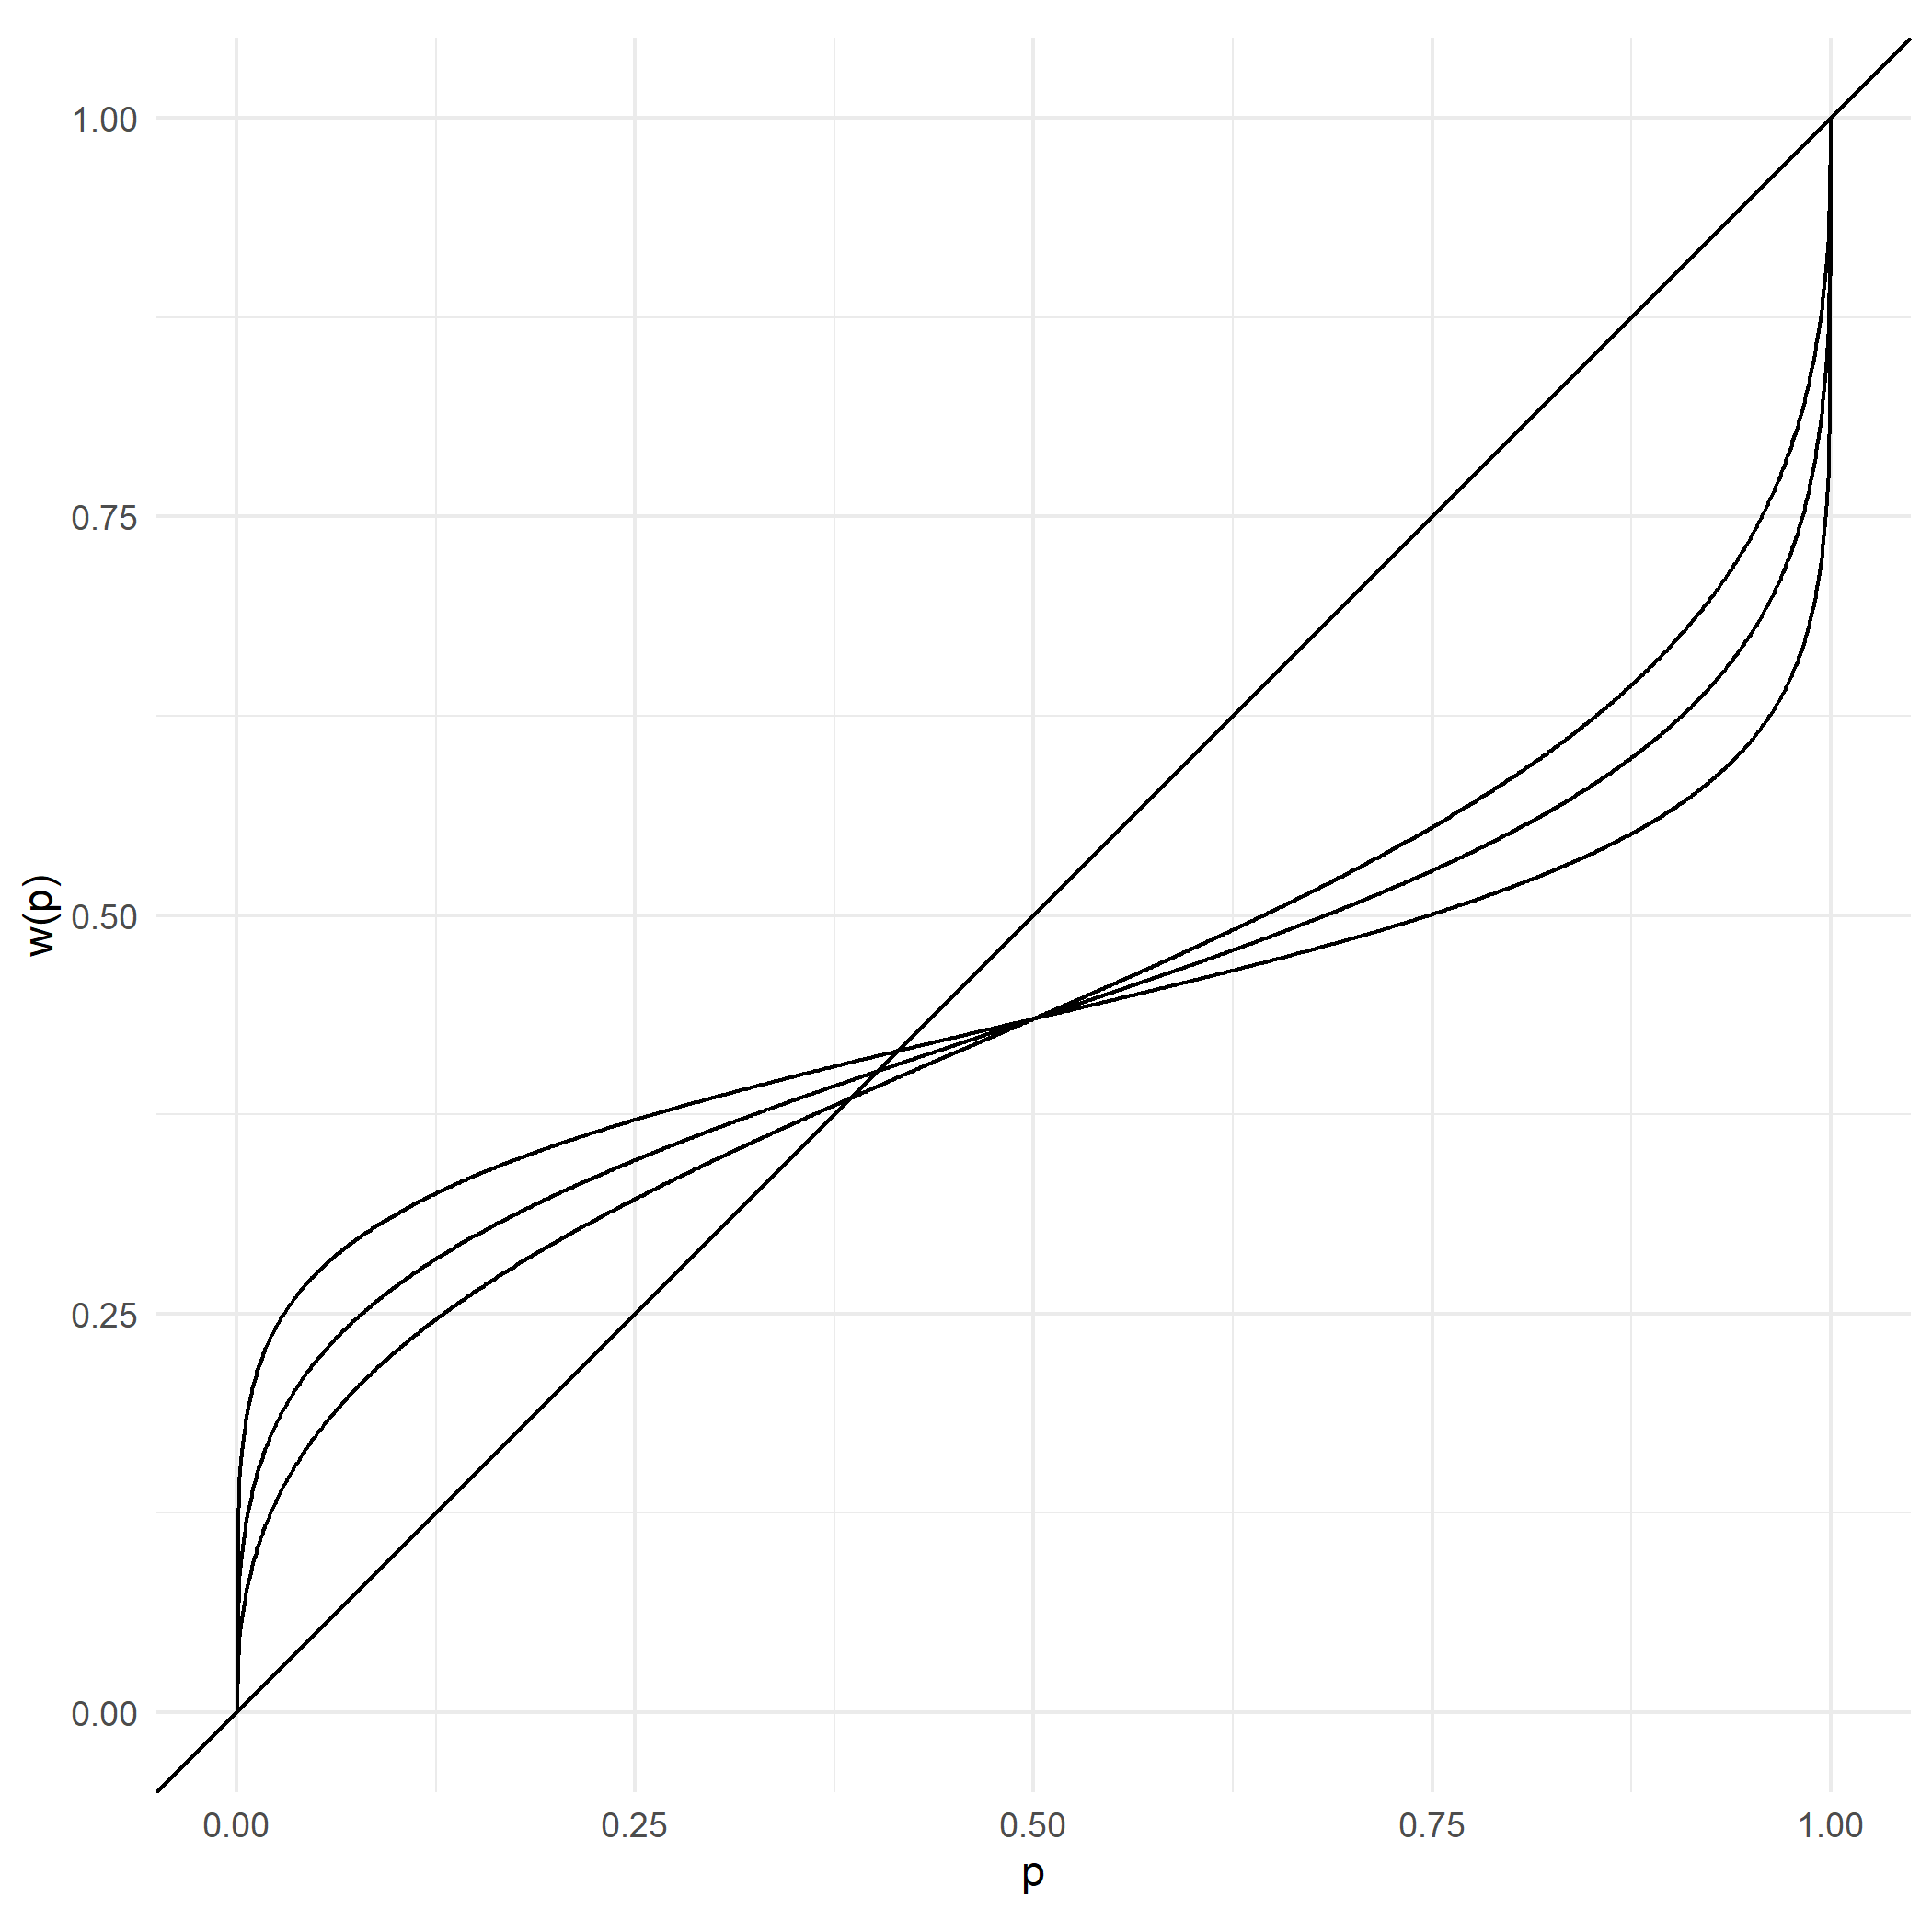
\includegraphics[width = \linewidth]{../Figures/ourHyp.png}
	\caption{For code, see
		\href{https://github.com/victor-m-p/BayesianDecisionWeights/blob/main/Code/0_visualize_parameters.Rmd}
		{this file} on
		\href{https://github.com/victor-m-p/BayesianDecisionWeights}{github}.
		Three curves shown, all with $\delta = 0.77$
	as reported in \textcite{gonzalez1999shape}.
	$\gamma$ levels $0.24, 0.34, 0.44$. The
	least curved line corresponds to $\gamma = 0.44$,
	as reported in \textcite{gonzalez1999shape}.
	For high-affect items $\gamma$ should
	be lower, and as such we suggest $0.24$
	(for high affect) and  $0.34$ (for medium
	affect) as minimally interesting effects
to detect.}
\end{figure}

\emph{Hypothesis 3:} No direction of effect
for the $\delta$ parameter by condition is
hypothesized. The  $\delta$ parameter is
not of interest to the main hypothesis
(replicating and extending \textcite{rottenstreich2001money})
and is mainly included in the analysis in
order to control for elevation so that the
$\gamma$ parameter can be estimated
properly. If the three items differ
in perceived overall value the $\delta$ parameter
should capture this. This means that our $\gamma$
distributions should still be interpretable
even if the $\delta$ parameter differs by
condition. The same analysis pipeline will be applied
to $\delta$ as for $\gamma$ (i.e. credibility
intervals obtained) but as suggested,
it is not clear whether an effect would
be interesting. The $\delta$ parameter is
expected to have a value close to $.77$
across conditions,
which is the population median found for
this parameter is \textcite{gonzalez1999shape}.

 \section{Design Plan}

\textbf{Study type:} Study 1 might be characterized
as an observational study, since it does not
really have an experimental manipulation. It
resembles a survey of questions (e.g. the 10
outcomes). Study 2 is an experiment using a
within-subjects design, in which all participants
participate in all three conditions ($A$,  $B$,  $C$).
This is important because within-subject designs
have better power to detect effects than
between-subject designs
\autocite{charness2012experimental}. Power is a
primary concern because effects are likely
to be small, and variance is likely to be high
\autocite{gonzalez1999shape}. A between-subjects
design is not necessary in our case, because we do
not induce an effect by priming, as in e.g.
\textcite{hsee2004music}. \\

\textbf{Blinding:} No blinding is involved in this study. \\

\subsection{Study Design}

\emph{Study 1}: All subjects will rate all 10 items
(see \emph{Appendix A}) as to the level of affect they
feel with regards to them. \\

\emph{Study 2}: All participants
indicate their certainty equivalence (CE) for all
certainty levels $p = 0.01, 0.03, \ldots, 0.99 \: (n = 50)$
and in all three conditions ($A$,  $B$,  $C$).
This results in $150$ observations per participant,
and  $50$ observations per participant for each
condition.

\section{Sampling Plan}

\textbf{Existing Data}: Registration prior
to creation of data. Data from simulation
does exist (see below \& at
\href{https://github.com/victor-m-p/BayesianDecisionWeights}{github}). \\

\textbf{Data collection procedures}:
Participants will be recruited through online
channels (e.g. facebook, student groups, etc.).
Participants must be at least 18 years old to
participate. In the first experiments subjects
will be payed $30$ DKK (or $\$5$)
for agreeing to participate
in an approx. $10$ minute online survey. In the
second experiment subjects will be payed $150$ DKK
(or $\$25$)
for agreeing to participate in an approx. $60$ minute
online experiment. \\

\textbf{Sample size}:

$30$ participants are recruited in both experiments
as a minimum. Depending on funds, more than $30$
participants would be preferable in especially
\emph{study 2} as this would
enable us to better estimate parameters. \\

\textbf{Sample size rationale}:

\emph{Study 1}: Data was simulated to estimate the
approximate sample size needed to obtain
a significant result from a paired t-test
between $A$ and  $B$ and between $B$ and  $C$.
Plotting and common
sense was used to arrive at best guesses for
reasonable values. Three distributions were generated

\begin{equation} \label{eq3}
\begin{split}
	item_A &\sim norm(0.2, 0.4) \\
	item_B &\sim norm(0.5, 0.4) \\
	item_C &\sim norm(0.8, 0.4)
\end{split}
\end{equation}

With $n = 30$ participants we have extremely
high power to detect these effects with a
one-tailed t-test (see
\href{https://github.com/victor-m-p/BayesianDecisionWeights/blob/main/Code/simulate_study1.Rmd}{this
file} on \href{https://github.com/victor-m-p/BayesianDecisionWeights}{github}). However,
as this is a cheap experiment to run, and the
results are critical for the second study
(it is important that the three best items are
used as the conditions in experiment 2)
this is thought reasonable.

\vspace{3mm}

\emph{Study 2}: Choice of sample
size is naturally related to
power. Typically, $.8$ power is considered reasonable
\autocite{cohen1992power},
although this is just convention. Power reflects the
ability to detect a effect and is influenced by
effect size and number of participants.
Unfortunately, a power simulation was not possible
to carry out since reasonable estimates for the
distributions (and effect sizes) are not present.
Additionally, there is no null hypothesis which
needs a significant/not-significant label (as
in a frequentist framework). Clearly, we need
power to detect effects that are interesting,
but several gradations of evidence are interesting.
For instance, if $.95$ credibility intervals do overlap
between conditions,
then the somewhat weaker result that  $.66$
credibility intervals do not overlap is still
interesting.
The simulation presented below likely underestimates
individual variation, which will lessen power.
The best comparison that we have is
\textcite{gonzalez1999shape} who estimate both
parameters of the value function $v$ as well
parameters $\gamma$ and  $\delta$ of the weighting
function  $w$. They do so with  $10$ participants and
collect data with respect to $15$ gambles crossed
with  $11$ probability levels \autocite{gonzalez1999shape}.
The fact that they are able to reasonably recover
the unobserved parameters (of  $v$ as well) with
a sample size of only $10$ participants suggests
that it is not so much the number of participants,
but rather the number of trials for each participant
that is important. Generally there is much
variation at the individual level
\autocite{gonzalez1999shape,
wu1996curvature,
abdellaoui2010separating}.
Based on the results of
\textcite{gonzalez1999shape}
and on the simulation carried
out, it is argued that $30$ participants should
probably give us reasonable power to detect
minimally interesting effects.

\section{Variables}

\subsection{Manipulated variables}

\emph{Study 1}: the only manipulated
variable is the difference in outcome
of the 10 different questions (see \emph{Appendix A}).
However, no a priori hypothesis as to which
outcomes elicit high affect is necessary,
and as such the experiment can be seen as
close in nature to an observational survey. \\

\emph{Study 2}: $50$ levels of uncertainty are
crossed with  $3$ conditions (different gambles).
These are the two manipulated variables of
study 2.

\subsection{Measured variables}

\emph{Study 1}: The single outcome variable
will be the rating of affect level. This will
be measured on a scale of $0-1$. Participants
will rate this using a slider (and will not see
the same scale that we measure). \\

\emph{Study 2}: The single outcome variable
is the price that subjects indicate that they
are willing to pay for a ticket in a lottery.
This measures the certainty equivalence (CE) of
participants, and can be thought of as $w(p)$.
This will be measured on a scale of $0-500$ dollars
using a slider. The max is 500 dollars since the
lottery tickets by definition cannot be worth
more than this.

\subsection{Indices}

No indices are used.

\section{Analysis Plan}

All analysis is performed in the programming
language \emph{R} \autocite{rcore} using
\emph{Rstudio} IDE
\autocite{rstudio}. A key package used for
bayesian model fitting is \emph{brms}
\autocite{brms}. \\

\emph{Study 1}: The measured affect ratings will be
ordered based on group-level means. The
three questions that best cover the affect-spectrum
are selected (explained earlier). The three items
are validated as being significantly different
with a paired (one-tailed) t-test.

\subsection{Simulation}

\emph{Study 2}: In order to test the pipeline for the
bayesian analysis, data simulation was
conducted. Unfortunately, \textcite{gonzalez1999shape}
do not exactly report the values (i.e.
distributional properties of $\tau$ and
$\gamma$) that we need
to generate data consistent with what they
gathered. As such, it does not make sense
to calculate power based on our simulations,
and the simulation serves the sole purpose
of making clear how analysis on eventual data
will be conducted. \\

Data is generated for $50$ probability levels,
$p = 0.01, 0.03,  \ldots, 0.99$ crossed with $3$
conditions, corresponding to the actual data
that will be collected.
Data is generated for $30$ simulated subjects (ID). \\

Note that standard deviations (noise) vary
between $\gamma$ and $\delta$, and at
different levels in our simulation. This qualitatively
follows the results of \textcite{gonzalez1999shape}.
Data is generated as a distribution of $\gamma$
and $\delta$ for each condition. We generate
$30$ values (i) for each, corresponding to the
number of participants. As we do not hypothesize
that $\delta$ is modulated by condition
this can simply be generated as once.
\begin{equation} \label{eq1}
\begin{split}
	\gamma_{A_{i}} &\sim norm(n = 30,
	m = 0.44, sd = 0.1) \\
	\gamma_{B_{i}} &\sim norm(n = 30,
	m = 0.34, sd = 0.1) \\
	\gamma_{C_{i}} &\sim norm(n = 30,
	m = 0.24, sd = 0.1) \\
	\delta_i &\sim norm(n = 90,
	m = 0.77, sd = 0.2)
\end{split}
\end{equation}

Based on these $\gamma$ and $\delta$ values for
participants per condition, we generate
the final $\gamma$ and $\delta$ values by
adding individual noise for each probability
level (j)
\begin{equation} \label{eq2}
\begin{split}
	\gamma_{A_{ij}} &\sim norm(n = 50,
	m = \gamma_{A_{i}}, sd = 0.1) \\
	\gamma_{B_{ij}} &\sim norm(n = 50,
	m = \gamma_{B_{i}}, sd = 0.1) \\
	\gamma_{C_{ij}} &\sim norm(n = 50,
	m = \gamma_{C_{i}}, sd = 0.1) \\
	\delta_{ij} &\sim norm(n = 150,
	m = \delta_{i}, sd = 0.3)
\end{split}
\end{equation}

As such, each condition will contain
two levels of noise around a true signal,
where the true population signal for
$\gamma$ varies by condition. For simulation
code see
\href{https://github.com/victor-m-p/BayesianDecisionWeights/blob/main/Code/1_simulate_data.Rmd}{this
file} on \href{https://github.com/victor-m-p/BayesianDecisionWeights}{my
github}.
The simulated data, and the best fit
$w(p)$ curves are shown in figure 4.
As can be seen, the simulated data shows
the expected pattern, where low values of
$\gamma$ exhibit more curvature. The preference
reversal shown in \textcite{rottenstreich2001money}
is also seen in the plot.

\begin{figure}[H]
	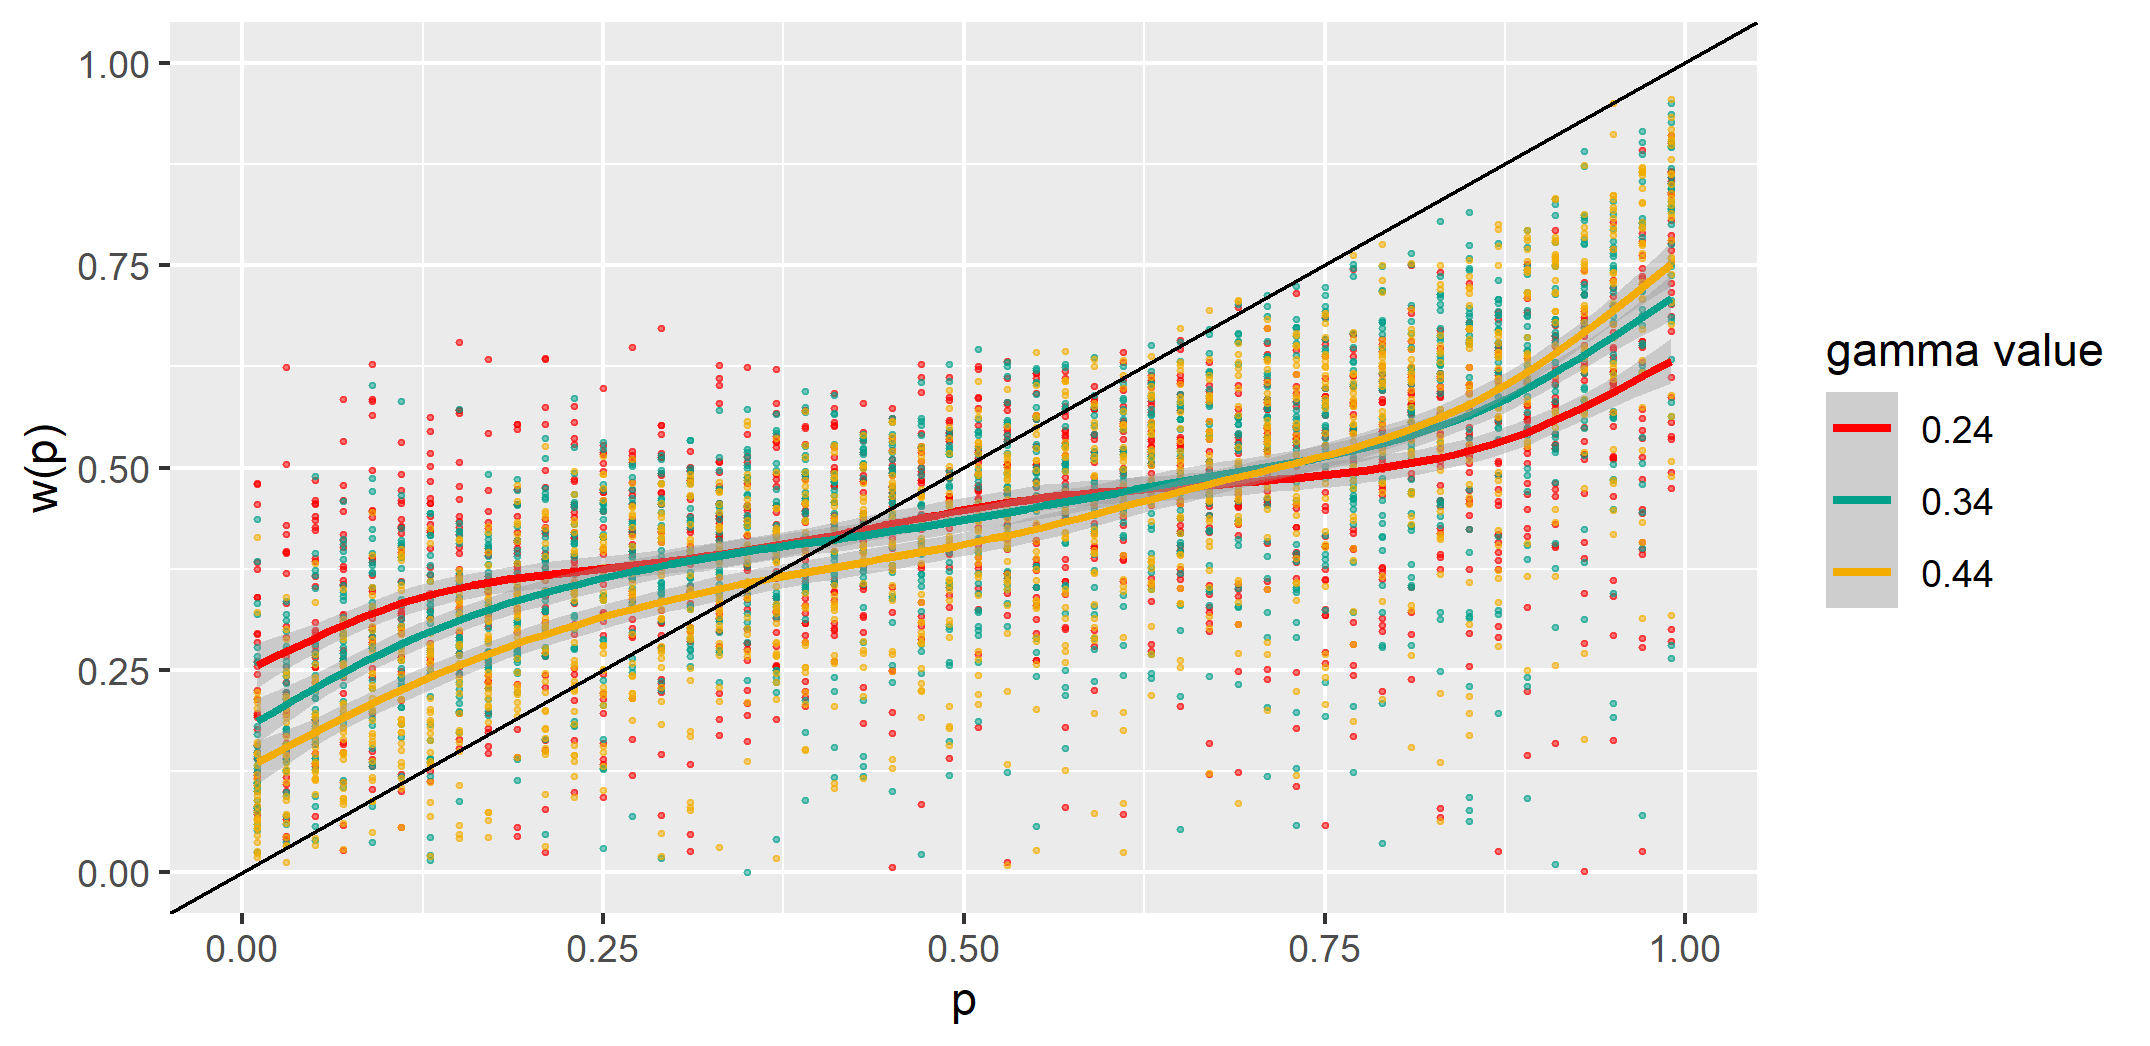
\includegraphics[width = \linewidth]{../Figures/simulated.png}
	\caption{Plot of simulated data in three
		conditions. $A \: (yellow)$ has
		$\gamma = 0.44$,
		$B \: (green)$ has $\gamma = 0.34$ and
		$C \: (red)$ has $\gamma = 0.24$.
		In all conditions
		the true population mean of
		$\delta = 0.77$. Shows the preference
		reversal observed in
	\textcite{rottenstreich2001money}. Note
	that the yellow curve corresponds
	roughly to what was found in
	\textcite{gonzalez1999shape}.
	The population effect is a
	weak, but true signal, which is
what we expect from the real data. Code for the figure in
		\href{https://github.com/victor-m-p/BayesianDecisionWeights/blob/main/Code/2_check_simulated.Rmd}{this
		file} on
		\href{https://github.com/victor-m-p/BayesianDecisionWeights}{the github}}.
\end{figure}

Next, the model described earlier is fitted
to the data (See
\href{https://github.com/victor-m-p/BayesianDecisionWeights/blob/main/Code/3_toy_model.Rmd}{this
file} on \href{https://github.com/victor-m-p/BayesianDecisionWeights}{the
github}). Regularizing riors are specified:
\[
	\tau \sim normal(0, 1)
\]
\[
	\gamma \sim normal(0.3, 0.5)
\]

They reflect our knowledge of reasonable values for
these parameters following both theory, and
experimental results \autocite{gonzalez1999shape}.
The same priors will be used for
modeling the actual data. Various characteristics,
such as R-hat and pp\_checks (from \emph{brms})
indicate a good model fit for the simulated data. \\

\begin{figure}[H]
	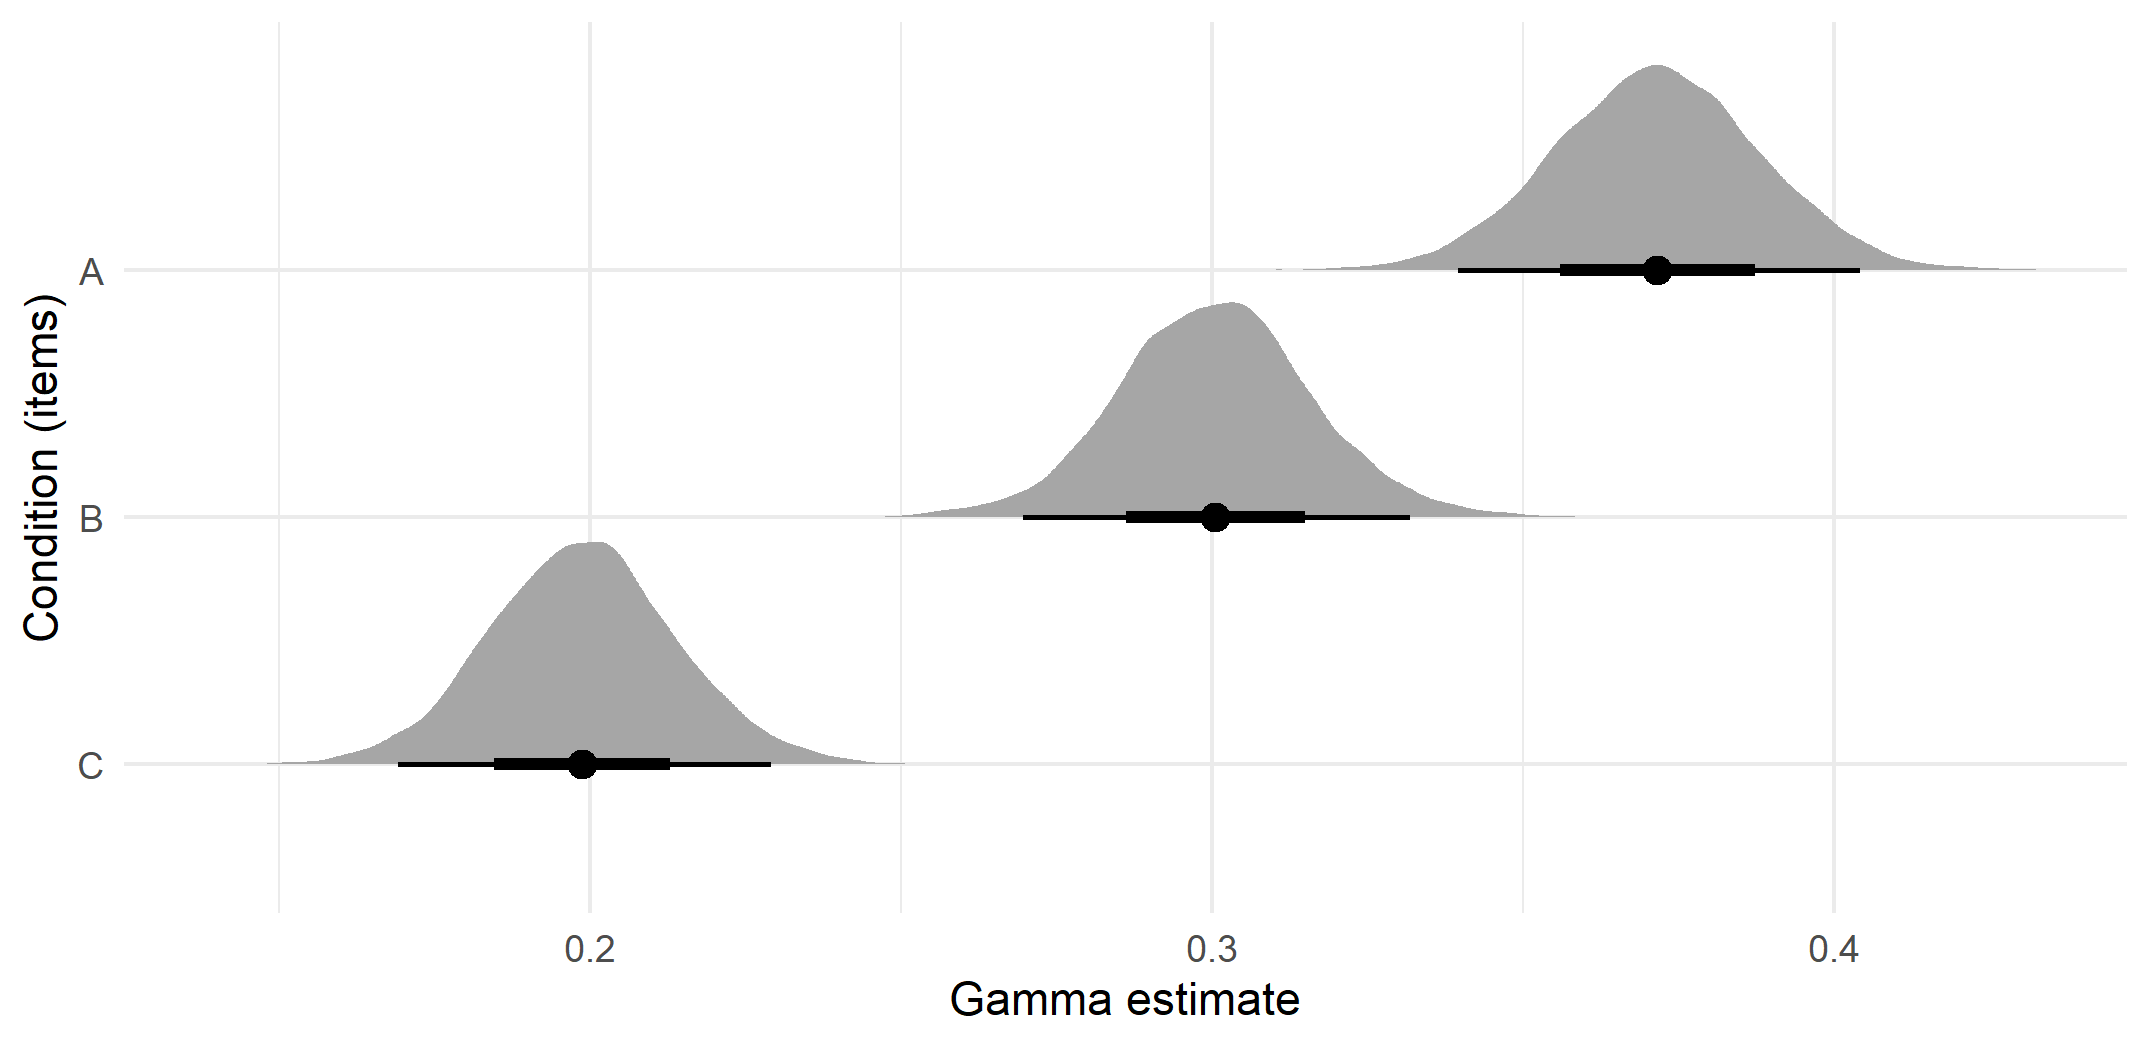
\includegraphics[width = \linewidth]{../Figures/gamma.png}
	\caption{showing the estimated  $\gamma$
	population distributions. The thick
	black line shows  $.66$ credibility intervals
	whereas the thin black line shows  $0.95$
	credibility intervals. Note that the
	conditions are ordered as expected with
	 $A$ having the highest  $\gamma$ and
	 $C$ having the lowest  $\gamma$.
	 Note that the  $.95$ credibility
	 intervals do not overlap. Code can
 be found in
 \href{https://github.com/victor-m-p/BayesianDecisionWeights/blob/main/Code/4_testing_hypotheses.Rmd}{this
 file} on \href{https://github.com/victor-m-p/BayesianDecisionWeights}{the
 github}}
 \end{figure}

We extract credibility intervals with regards
to $\gamma$ and $\delta$ distributions for each
condition ($A$, $B$, $C$). With the simulated
data, we note that the model is capable of
recovering the unobserved (unmeasured) parameters,
and that for $\gamma$ the  $.95$ credibility
intervals do not overlap between conditions
(see figure 5). The estimates and credibility intervals
are, $\gamma_{A} = 0.37, \: CI: [0.34, 0.40]$,
$\gamma_{B} = 0.30, \: CI: [0.27, 0.33]$ and
$\gamma_{C} = 0.20, \: CI: [0.17, 0.23]$.
This slightly underestimates the true effect, which
we know because we simulated the data. However, it
is reasonably close. This shows that with $30$
participants, and 50 probability levels crossed with
3 conditions it is possible to detect the effect
that we are interested in. This of course assumes specific
distributional characteristics and noise-levels
that we cannot know in advance. It does however, show
that the model and the pipeline works as intended.

\section{Discussion \& Future Work}

The two-part study presented here is important
for several reasons. Firstly, it attempts to
formalize an interesting finding in the
field of decision making (DM). The author
strongly believe that formalization is the way to
make DM and psychology generally a more
reproducible and predictive science.
The effect that this study tries to replicate
\autocite{rottenstreich2001money} is
very interesting. However, the study
bases the claim that the
probability weighting function $w$ is
modulated by affect on of a measurement of end-points
($1\%$ and $99\%$) only.
As such, it is rather stylized; i.e. they
are not able to estimate the modulation of
the actual parameters of the weighting function
based on their experiment.
It is surprising that no-one (to my knowledge)
has actually followed the suggestion
of \autocite{rottenstreich2001money} in extending
their stylized effect. Testing it for more than
two items and across enough uncertainty
levels to estimate parameters of the weighting
function $w$ seems like a worthwile effort.

\vspace{3mm}
The present study also attempts to facilitate
cumulative science more generally, by providing
all code, simulation and eventual data at
\href{https://github.com/victor-m-p/BayesianDecisionWeights}
{github}.
By making the code and data accessible, future
experimenters can use the knowledge obtained in
this experiment to motivate stronger priors in
subsequent experiments. This effectively
pools information across studies
(i.e. our posterior becomes their prior). Sadly,
most of the research in this area is carried
out in a frequentist framework
\autocite{gonzalez1999shape, rottenstreich2001money,
hsee2004music}, and often
code and data is not accessible. This makes it
impossible to properly integrate previous work
and thus achieve a truly cumulative scientific effort.

\vspace{3mm}
If the current two-part study is successful,
there are several obvious avenues of further
work. Specifically, the boundaries of the modulatory
effect of affect should be investigated. The
proposed study
only uses gambles in the gains domain (i.e. "how
much would you be willing to pay for a
certain probability of winning something?")
and as such it only models $w^{+}$. To model
$w^{-}$, a similar
study could be run for the loss domain, still with
validated high-affect and low-affect items (i.e. "how
much would you be willing to pay to avoid a
certain probability of loosing something/something
bad happening?"). It has been experimentally
found that subjets are more sensitive to
probabilities of gains ($w^{+}$) than
losses ($w^{-}$) \autocite{
abdellaoui2010separating} but whether there is a
modulatory effect of affect-richness is unclear.\\

A second avenue of further study is to broaden
the analysis to include estimation of paramters
of both the value function $v$ and the weight
function  $w$. This would be interesting because
the stylized effects of \textcite{
rottenstreich2001money} and \textcite{hsee2004music}
could be tested together. This could validate
the coherent picture of affective modulation
of both $v$ and  $w$ that
these two papers seem to suggest in
conjunction. \\

Lastly, this study assumes
a specific parameterization of
the probability weighting function $w$.
Non-parametric approaches which do not assume
specific functions exist, and it can
be argued that these should be preferred
as long as there is not agreement as to
the correct functional form of the
probability weighting function
\autocite{wu1996curvature}.

\printbibliography
\section{Appendix}

\emph{Appendix A} \\
As all items in study 1 follow the same template: \\

"If you won a $\$500$ coupon redeemable for/at
$[x]$ how emotionally affected would you be?" \\

The $10$ proposed $[x]$ outcomes are:
\begin{itemize}
	\item for a vacation abroad with a friend/partner.
	\item at a local shopping mall.
	\item for donation to a charity of your choice.
	\item for a cultural experience in your city.
	\item for insurance covering.
	\item for investing in the stock market.
	\item for job training.
	\item for $\$500$.
	\item for spending on a present to someone you love.
	\item at your favorite restaurant.
\end{itemize}

\end{document}


